% future/tm.tex

\section{Transactional Memory}
\label{sec:future:Transactional Memory}

The idea of using transactions outside of databases goes back many
decades~\cite{DBLomet1977SIGSOFT}, with the key difference between
database and non-database transactions being that non-database transactions
drop the ``D'' in the ``ACID'' properties defining database transactions.
The idea of supporting memory-based transactions, or ``transactional memory''
(TM), in hardware
is more recent~\cite{Herlihy93a}, but unfortunately, support for such
transactions in commodity hardware was not immediately forthcoming,
despite other somewhat similar proposals being put forward~\cite{JMStone93}.
Not long after, Shavit and Touitou proposed a software-only implementation
of transactional memory (STM) that was capable of running on commodity
hardware, give or take memory-ordering issues.
This proposal languished for many years, perhaps due to the fact that
the research community's attention was absorbed by non-blocking
synchronization (see Section~\ref{sec:advsync:Non-Blocking Synchronization}).

But by the turn of the century, TM started receiving
more attention~\cite{Martinez01a,Rajwar01a}, and by the middle of the
decade, the level of interest can only be termed
``incandescent''~\cite{MauriceHerlihy2005-TM-manifesto.pldi,
DanGrossman2007TMGCAnalogy}, despite a few voices of
caution~\cite{Blundell2005DebunkTM,McKenney2007PLOSTM}.

The basic idea behind TM is to execute a section of
code atomically, so that other threads see no intermediate state.
As such, the semantics of TM could be implemented
by simply replacing each transaction with a recursively acquirable
global lock acquisition and release, albeit with abysmal performance
and scalability.
Much of the complexity inherent in TM implementations, whether hardware
or software, is efficiently detecting when concurrent transactions can safely
run in parallel.
Because this detection is done dynamically, conflicting transactions
can be aborted or ``rolled back'', and in some implementations, this
failure mode is visible to the programmer.

Because transaction roll-back is increasingly unlikely as transaction
size decreases, TM might become quite attractive for small memory-based
operations,
such as linked-list manipulations used for stacks, queues, hash tables,
and search trees.
However, it is currently much more difficult to make the case for large
transactions, particularly those containing non-memory operations such
as I/O and process creation.
The following sections look at current challenges to the grand vision of
``Transactional Memory Everywhere''~\cite{PaulEMcKenney2009TMeverywhere}.
Section~\ref{sec:future:Outside World} examines the challenges faced
interacting with the outside world,
Section~\ref{sec:future:Process Modification} looks at interactions
with process modification primitives,
Section~\ref{sec:future:Synchronization} explores interactions with
other synchronization primitives, and finally
Section~\ref{sec:future:Discussion} closes with some discussion.

\subsection{Outside World}
\label{sec:future:Outside World}

In the words of Donald Knuth:

\begin{quote}
	Many computer users feel that input and output are not actually part
	of ``real programming,'' they are merely things that (unfortunately)
	must be done in order to get information in and out of the machine.
\end{quote}

Whether we believe that input and output are ``real programming'' or
not, the fact is that for most computer systems, interaction with the
outside world is a first-class requirement.
This section therefore critiques transactional memory's ability to
so interact, whether via I/O operations, time delays, or persistent
storage.

\subsubsection{I/O Operations}
\label{sec:future:I/O Operations}

One can execute I/O operations within a lock-based critical section,
and, at least in principle, from within an RCU read-side critical section.
What happens when you attempt to execute an I/O operation from within
a transaction?

The underlying problem is that transactions may be rolled back, for
example, due to conflicts.
Roughly speaking, this requires that all operations within any given
transaction be revocable, so that executing the operation twice has
the same effect as executing it once.
Unfortunately, I/O is in general the prototypical irrevocable
operation, making it difficult to include general I/O operations in
transactions.
In fact, general I/O is irrevocable:
Once you have pushed the button launching the nuclear warheads, there
is no turning back.

Here are some options for handling of I/O within transactions:

\begin{enumerate}
\item	Restrict I/O within transactions to buffered I/O with in-memory
	buffers.
	These buffers may then be included in the transaction in the
	same way that any other memory location might be included.
	This seems to be the mechanism of choice, and it does work
	well in many common cases of situations such as stream I/O and
	mass-storage I/O.
	However, special handling is required in cases where multiple
	record-oriented output streams are merged onto a single file
	from multiple processes, as might be done using the ``a+''
	option to \co{fopen()} or the \co{O_APPEND}  flag to \co{open()}.
	In addition, as will be seen in the next section, common
	networking operations cannot be handled via buffering.
\item	Prohibit I/O within transactions, so that any attempt to execute
	an I/O operation aborts the enclosing transaction (and perhaps
	multiple nested transactions).
	This approach seems to be the conventional TM approach for
	unbuffered I/O, but requires that TM interoperate with other
	synchronization primitives that do tolerate I/O.
\item	Prohibit I/O within transactions, but enlist the compiler's aid
	in enforcing this prohibition.
\item	Permit only one special
	\emph{irrevocable} transaction~\cite{SpearMichaelScott2008InevitableSTM}
	to proceed
	at any given time, thus allowing irrevocable transactions to
	contain I/O operations.\footnote{
		In earlier literature, irrevocable transactions are
		termed \emph{inevitable} transactions.}
	This works in general, but severely limits the scalability and
	performance of I/O operations.
	Given that scalability and performance is a first-class goal of
	parallelism, this approach's generality seems a bit self-limiting.
	Worse yet, use of irrevocability to tolerate I/O operations
	seems to prohibit use of manual transaction-abort operations.\footnote{
		This difficulty was pointed out by Michael Factor.}
	Finally, if there is an irrevocable transaction manipulating
	a given data item, any other transaction manipulating that
	same data item cannot have non-blocking semantics.
\item	Create new hardware and protocols such that I/O operations can
	be pulled into the transactional substrate.
	In the case of input operations, the hardware would need to
	correctly predict the result of the operation, and to abort the
	transaction if the prediction failed.
\end{enumerate}

I/O operations are a well-known weakness of TM, and it is not clear
that the problem of supporting I/O in transactions has a reasonable
general solution, at least if ``reasonable'' is to include usable
performance and scalability.
Nevertheless, continued time and attention to this problem will likely
produce additional progress.

\subsubsection{RPC Operations}
\label{sec:future:RPC Operations}

One can execute RPCs within a lock-based critical section, as well as
from within an RCU read-side critical section. What happens when you
attempt to execute an RPC from within a transaction?

If both the RPC request and its response are to be contained within the
transaction, and if some part of the transaction depends on the result
returned by the response, then it is not possible to use the memory-buffer
tricks that can be used in the case of buffered I/O.
Any attempt to
take this buffering approach would deadlock the transaction, as the
request could not be transmitted until the transaction was guaranteed
to succeed, but the transaction's success might not be knowable until
after the response is received, as is the case in the following example:

\vspace{5pt}
\begin{minipage}[t]{\columnwidth}
\small
\begin{verbatim}
  1 begin_trans();
  2 rpc_request();
  3 i = rpc_response();
  4 a[i]++;
  5 end_trans();
\end{verbatim}
\end{minipage}
\vspace{5pt}

The transaction's memory footprint cannot be determined until after the
RPC response is received, and until the transaction's memory footprint
can be determined, it is impossible to determine whether the transaction
can be allowed to commit.
The only action consistent with transactional semantics is therefore to
unconditionally abort the transaction, which is, to say the least,
unhelpful.

Here are some options available to TM:

\begin{enumerate}
\item	Prohibit RPC within transactions, so that any attempt to execute
	an RPC operation aborts the enclosing transaction (and perhaps
	multiple nested transactions).
	Alternatively, enlist the compiler to enforce RPC-free
	transactions.
	This approach does work, but will require TM to
	interact with other synchronization primitives.
\item	Permit only one special
	irrevocable transaction~\cite{SpearMichaelScott2008InevitableSTM}
	to proceed at any given time, thus allowing irrevocable
	transactions to contain RPC operations.
	This works in general, but severely limits the scalability and
	performance of RPC operations.
	Given that scalability and performance is a first-class goal of
	parallelism, this approach's generality seems a bit self-limiting.
	Furthermore, use of irrevocable transactions to permit RPC
	operations rules out manual transaction-abort operations
	once the RPC operation has started.
	Finally, if there is an irrevocable transaction manipulating
	a given data item, any other transaction manipulating that
	same data item cannot have non-blocking semantics.
\item	Identify special cases where the success of the transaction may
	be determined before the RPC response is received, and
	automatically convert these to irrevocable transactions immediately
	before sending the RPC request.
	Of course, if several concurrent transactions attempt RPC calls
	in this manner, it might be necessary to roll all but one of them
	back, with consequent degradation of performance and scalability.
	This approach nevertheless might be valuable given long-running
	transactions ending with an RPC.
	This approach still has problems with manual transaction-abort
	operations.
\item	Identify special cases where the RPC response may be moved out
	of the transaction, and then proceed using techniques similar
	to those used for buffered I/O.
\item	Extend the transactional substrate to include the RPC server as
	well as its client.
	This is in theory possible, as has been demonstrated by
	distributed databases.
	However, it is unclear whether the requisite performance and
	scalability requirements can be met by distributed-database
	techniques, given that memory-based TM cannot hide such latencies
	behind those of slow disk drives.
	Of course, given the advent of solid-state disks, it is also unclear
	how much longer databases will be permitted to hide their latencies
	behind those of disks drives.
\end{enumerate}

As noted in the prior section, I/O is a known weakness of TM, and RPC
is simply an especially problematic case of I/O.

\subsubsection{Time Delays}
\label{sec:future:Time Delays}

An important special case of interaction with extra-transactional accesses
involves explicit time delays within a transaction.
Of course, the idea of a time delay within a transaction flies in the
face of TM's atomicity property, but one can argue that this sort of
thing is what weak atomicity is all about.
Furthermore, correct interaction with memory-mapped I/O sometimes requires
carefully controlled timing, and applications often use time delays
for varied purposes.

So, what can TM do about time delays within transactions?

\begin{enumerate}
\item	Ignore time delays within transactions.
	This has an appearance of elegance, but like too many other
	``elegant'' solutions, fails to survive first contact with
	legacy code.
	Such code, which might well have important time delays in critical
	sections, would fail upon being transactionalized.
\item	Abort transactions upon encountering a time-delay operation.
	This is attractive, but it is unfortunately not always possible
	to automatically detect a time-delay operation.
	Is that tight loop computing something important, or is it
	instead waiting for time to elapse?
\item	Enlist the compiler to prohibit time delays within transactions.
\item	Let the time delays execute normally.
	Unfortunately, some TM implementations publish modifications only
	at commit time, which would in many cases defeat the purpose of
	the time delay.
\end{enumerate}

It is not clear that there is a single correct answer.
TM implementations featuring weak atomicity that publish changes
immediately within the transaction (rolling these changes back upon abort)
might be reasonably well served by the last alternative.
Even in this case, the code (or possibly even hardware) at the other
end of the transaction may require a substantial redesign to tolerate
aborted transactions.
This need for redesign would make it more difficult to apply transactional
memory to legacy code.

\subsubsection{Persistence}
\label{sec:future:Persistence}

There are many different types of locking primitives.
One interesting distinction is persistence, in other words, whether the
lock can exist independently of the address space of the process using
the lock.

Non-persistent locks include \co{pthread_mutex_lock()},
\co{pthread_rwlock_rdlock()}, and most kernel-level locking primitives.
If the memory locations instantiating a non-persistent lock's data
structures disappear, so does the lock.
For typical use of \co{pthread_mutex_lock()}, this means that when the
process exits, all of its locks vanish.
This property can be exploited in order to trivialize lock cleanup
at program shutdown time, but makes it more difficult for unrelated
applications to share locks, as such sharing requires the applications
to share memory.

Persistent locks help avoid the need to share memory among unrelated
applications.
Persistent locking APIs include the flock family, \co{lockf()}, System
V semaphores, or the \co{O_CREAT} flag to \co{open()}.
These persistent APIs can be used to protect large-scale operations
spanning runs of multiple applications, and, in the case of \co{O_CREAT}
even surviving operating-system reboot.
If need be, locks can even span multiple computer systems via distributed
lock managers and distributed filesystems---and persist across reboots
of any or all of these computer systems.

Persistent locks can be used by any application, including applications
written using multiple languages and software environments.
In fact, a persistent lock might well be acquired by an application written
in C and released by an application written in Python.

How could a similar persistent functionality be provided for TM?

\begin{enumerate}
\item	Restrict persistent transactions to special-purpose environments
	designed to support them, for example, SQL.
	This clearly works, given the decades-long history of database
	systems, but does not provide the same degree of flexibility
	provided by persistent locks.
\item	Use snapshot facilities provided by some storage devices and/or
	filesystems.
	Unfortunately, this does not handle network communication,
	nor does it handle I/O to devices that do not provide snapshot
	capabilities, for example, memory sticks.
\item	Build a time machine.
\end{enumerate}

Of course, the fact that it is called transactional \emph{memory}
should give us pause, as the name itself conflicts with the concept of
a persistent transaction.
It is nevertheless worthwhile to consider this possibility as an important
test case probing the inherent limitations of transactional memory.

\subsection{Process Modification}
\label{sec:future:Process Modification}

Processes are not eternal:
They are created and destroyed, their memory mappings are modified,
they are linked to dynamic libraries, and they are debugged.
These sections look at how transactional memory can handle an
ever-changing execution environment.

\subsubsection{Multithreaded Transactions}
\label{sec:future:Multithreaded Transactions}

It is perfectly legal to create processes and threads while holding
a lock or, for that matter, from within an RCU read-side critical
section.
Not only is it legal, but it is quite simple, as can be seen from the
following code fragment:

\vspace{5pt}
\begin{minipage}[t]{\columnwidth}
\small
\begin{verbatim}
  1 pthread_mutex_lock(...);
  2 for (i = 0; i < ncpus; i++)
  3   pthread_create(&tid[i], ...);
  4 for (i = 0; i < ncpus; i++)
  5   pthread_join(tid[i], ...);
  6 pthread_mutex_unlock(...);
\end{verbatim}
\end{minipage}
\vspace{5pt}

This pseudo-code fragment uses \co{pthread_create()} to spawn one thread
per CPU, then uses \co{pthread_join()} to wait for each to complete,
all under the protection of \co{pthread_mutex_lock()}.
The effect is to execute a lock-based critical section in parallel,
and one could obtain a similar effect using \co{fork()} and \co{wait()}.
Of course, the critical section would need to be quite large to justify
the thread-spawning overhead, but there are many examples of large
critical sections in production software.

What might TM do about thread spawning within a transaction?

\begin{enumerate}
\item	Declare \co{pthread_create()} to be illegal within transactions,
	resulting in transaction abort (preferred) or undefined
	behavior. Alternatively, enlist the compiler to enforce
	\co{pthread_create()}-free transactions.
\item	Permit \co{pthread_create()} to be executed within a
	transaction, but only the parent thread will be considered to
	be part of the transaction.
	This approach seems to be reasonably compatible with existing and
	posited TM implementations, but seems to be a trap for the unwary.
	This approach raises further questions, such as how to handle
	conflicting child-thread accesses.
\item	Convert the \co{pthread_create()}s to function calls.
	This approach is also an attractive nuisance, as it does not
	handle the not-uncommon cases where the child threads communicate
	with one another.
	In addition, it does not permit parallel execution of the body
	of the transaction.
\item	Extend the transaction to cover the parent and all child threads.
	This approach raises interesting questions about the nature of
	conflicting accesses, given that the parent and children are
	presumably permitted to conflict with each other, but not with
	other threads.
	It also raises interesting questions as to what should happen
	if the parent thread does not wait for its children before
	committing the transaction.
	Even more interesting, what happens if the parent conditionally
	executes \co{pthread_join()} based on the values of variables
	participating in the transaction?
	The answers to these questions are reasonably straightforward
	in the case of locking.
	The answers for TM are left as an exercise for the reader.
\end{enumerate}

Given that parallel execution of transactions is commonplace in the
database world, it is perhaps surprising that current TM proposals do
not provide for it.
On the other hand, the example above is a fairly sophisticated use
of locking that is not normally found in simple textbook examples,
so perhaps its omission is to be expected.
That said, there are rumors that some TM researchers are investigating
fork/join parallelism within transactions, so perhaps this topic will
soon be addressed more thoroughly.

\subsubsection{The exec() System Call}
\label{sec:future:The exec System Call}

One can execute an \co{exec()} system call while holding a lock, and
also from within an RCU read-side critical section.
The exact semantics depends on the type of primitive.

In the case of non-persistent primitives (including
\co{pthread_mutex_lock()}, \co{pthread_rwlock_rdlock()}, and RCU),
if the \co{exec()} succeeds, the whole address space vanishes, along
with any locks being held.
Of course, if the \co{exec()} fails, the address space still lives,
so any associated locks would also still live.
A bit strange perhaps, but reasonably well defined.

On the other hand, persistent primitives (including the flock family,
\co{lockf()}, System V semaphores, and the \co{O_CREAT} flag to
\co{open()}) would survive regardless of whether the \co{exec()}
succeeded or failed, so that the \co{exec()}ed program might well
release them.

\QuickQuiz{}
	What about non-persistent primitives represented by data
	structures in \co{mmap()} regions of memory?
	What happens when there is an \co{exec()} within a critical
	section of such a primitive?
\QuickQuizAnswer{
	If the \co{exec()}ed program maps those same regions of
	memory, then this program could in principle simply release
	the lock.
	The question as to whether this approach is sound from a
	software-engineering viewpoint is left as an exercise for
	the reader.
} \QuickQuizEnd

What happens when you attempt to execute an \co{exec()} system call
from within a transaction?

\begin{enumerate}
\item	Disallow \co{exec()} within transactions, so that the enclosing
	transactions abort upon encountering the \co{exec()}.
	This is well defined, but clearly requires non-TM synchronization
	primitives for use in conjunction with \co{exec()}.
\item	Disallow \co{exec()} within transactions, with the compiler
	enforcing this prohibition.
	There is a draft specification for TM in C++ that takes
	this approach, allowing functions to be decorated with
	the \co{transaction_safe} and \co{transaction_unsafe}
	attributes.\footnote{
		Thanks to Mark Moir for pointing me at this spec, and
		to Michael Wong for having pointed me at an earlier
		revision some time back.}
	This approach has some advantages over aborting the transaction
	at runtime, but again requires non-TM synchronization primitives
	for use in conjunction with \co{exec()}.
\item	Treat the transaction in a manner similar to non-persistent
	Locking primitives, so that the transaction survives if \co{exec()}
	fails, and silently commits if the \co{exec()} succeeds.
	The case where some of the variables affected by the transaction
	reside in \co{mmap()}ed memory (and thus could survive a successful
	\co{exec()} system call) is left as an exercise for the reader.
\item	Abort the transaction (and the \co{exec()} system call) if the
	\co{exec()} system call would have succeeded, but allow the
	transaction to continue if the \co{exec()} system call would
	fail.
	This is in some sense the ``correct'' approach, but it would
	require considerable work for a rather unsatisfying result.
\end{enumerate}

The \co{exec()} system call is perhaps the strangest example of an
obstacle to universal TM applicability, as it is not completely clear
what approach makes sense, and some might argue that this is merely a
reflection of the perils of interacting with execs in real life.
That said, the two options prohibiting \co{exec()} within transactions
are perhaps the most logical of the group.

Similar issues surround the \co{exit()} and \co{kill()} system calls.

\subsubsection{Dynamic Linking and Loading}
\label{sec:future:Dynamic Linking and Loading}

Both lock-based critical sections and RCU read-side critical sections
can legitimately contain code that invokes dynamically linked and loaded
functions, including C/C++ shared libraries and Java class libraries.
Of course, the code contained in these libraries is by definition
unknowable at compile time.
So, what happens if a dynamically loaded function is invoked within
a transaction?

This question has two parts: (a)~how do you dynamically link and load a
function within a transaction and (b)~what do you do about the unknowable
nature of the code within this function?
To be fair, item (b) poses some challenges for locking and RCU as well,
at least in theory.
For example, the dynamically linked function might introduce a deadlock
for locking or might (erroneously) introduce a quiescent state into an
RCU read-side critical section.
The difference is that while the class of operations permitted in locking
and RCU critical sections is well-understood, there appears to still be
considerable uncertainty in the case of TM.
In fact, different implementations of TM seem to have different restrictions.

So what can TM do about dynamically linked and loaded library functions?
Options for part (a), the actual loading of the code, include the following:

\begin{enumerate}
\item	Treat the dynamic linking and loading in a manner similar to a
	page fault, so that the function is loaded and linked, possibly
	aborting the transaction in the process.
	If the transaction is aborted, the retry will find the function
	already present, and the transaction can thus be expected to
	proceed normally.
\item	Disallow dynamic linking and loading of functions from within
	transactions.
\end{enumerate}

Options for part (b), the inability to detect TM-unfriendly operations
in a not-yet-loaded function, possibilities include the following:

\begin{enumerate}
\item	Just execute the code: if there are any TM-unfriendly operations
	in the function, simply abort the transaction.
	Unfortunately, this approach makes it impossible for the compiler
	to determine whether a given group of transactions may be safely
	composed.
	One way to permit composability regardless is irrevocable
	transactions, however, current implementations permit only a
	single irrevocable transaction to proceed at any given time,
	which can severely limit performance and scalability.
	Irrevocable transactions also seem to rule out use of manual
	transaction-abort operations.
	Finally, if there is an irrevocable transaction manipulating
	a given data item, any other transaction manipulating that
	same data item cannot have non-blocking semantics.
\item	Decorate the function declarations indicating which functions
	are TM-friendly.
	These decorations can then be enforced by the compiler's type system.
	Of course, for many languages, this requires language extensions
	to be proposed, standardized, and implemented, with the
	corresponding time delays.
	That said, the standardization effort is already in
	progress~\cite{Ali-Reza-Adl-Tabatabai2009CppTM}.
\item	As above, disallow dynamic linking and loading of functions from
	within transactions.
\end{enumerate}

I/O operations are of course a known weakness of TM, and dynamic linking
and loading can be thought of as yet another special case of I/O.
Nevertheless, the proponents of TM must either solve this problem, or
resign themselves to a world where TM is but one tool of several in the
parallel programmer's toolbox.
(To be fair, a number of TM proponents have long since resigned themselves
to a world containing more than just TM.)

\subsubsection{Memory-Mapping Operations}
\label{sec:future:Memory-Mapping Operations}

It is perfectly legal to execute memory-mapping operations (including
\co{mmap()}, \co{shmat()}, and \co{munmap()}~\cite{TheOpenGroup1997SUS})
within a lock-based critical section,
and, at least in principle, from within an RCU read-side critical section.
What happens when you attempt to execute such an operation from within
a transaction?
More to the point, what happens if the memory region being remapped
contains some variables participating in the current thread's transaction?
And what if this memory region contains variables participating in some
other thread's transaction?

It should not be necessary to consider cases where the TM system's
metadata is remapped, given that most locking primitives do not define
the outcome of remapping their lock variables.

Here are some memory-mapping options available to TM:

\begin{enumerate}
\item	Memory remapping is illegal within a transaction, and will result
	in all enclosing transactions being aborted.
	This does simplify things somewhat, but also requires that TM
	interoperate with synchronization primitives that do tolerate
	remapping from within their critical sections.
\item	Memory remapping is illegal within a transaction, and the
	compiler is enlisted to enforce this prohibition.
\item	Memory mapping is legal within a transaction, but aborts all
	other transactions having variables in the region mapped over.
\item	Memory mapping is legal within a transaction, but the mapping
	operation will fail if the region being mapped overlaps with
	the current transaction's footprint.
\item	All memory-mapping operations, whether within or outside a
	transaction, check the region being mapped against the memory
	footprint of all transactions in the system.
	If there is overlap, then the memory-mapping operation fails.
\item	The effect of memory-mapping operations that overlap the memory
	footprint of any transaction in the system is determined by the
	TM conflict manager, which might dynamically determine whether
	to fail the memory-mapping operation or abort any conflicting
	transactions.
\end{enumerate}

It is interesting to note that \co{munmap()} leaves the relevant region
of memory unmapped, which could have additional interesting
implications.\footnote{
	This difference between mapping and unmapping was noted by
	Josh Triplett.}

\subsubsection{Debugging}
\label{sec:future:Debugging}

The usual debugging operations such as breakpoints work normally within
lock-based critical sections and from RCU read-side critical sections.
However, in initial transactional-memory hardware
implementations~\cite{DaveDice2009ASPLOSRockHTM} an exception within
a transaction will abort that transaction, which in turn means that
breakpoints abort all enclosing transactions

So how can transactions be debugged?

\begin{enumerate}
\item	Use software emulation techniques within transactions containing
	breakpoints.
	Of course, it might be necessary to emulate all transactions
	any time a breakpoint is set within the scope of any transaction.
	If the runtime system is unable to determine whether or not a
	given breakpoint is within the scope of a transaction, then it
	might be necessary to emulate all transactions just to be on
	the safe side.
	However, this approach might impose significant overhead, which
	might in turn obscure the bug being pursued.
\item	Use only hardware TM implementations that are capable of
	handling breakpoint exceptions.
	Unfortunately, as of this writing (September 2008), all such
	implementations are strictly research prototypes.
\item	Use only software TM implementations, which are
	(very roughly speaking) more tolerant of exceptions than are
	the simpler of the hardware TM implementations.
	Of course, software TM tends to have higher overhead than hardware
	TM, so this approach may not be acceptable in all situations.
\item	Program more carefully, so as to avoid having bugs in the
	transactions in the first place.
	As soon as you figure out how to do this, please do let everyone
	know the secret!
\end{enumerate}

There is some reason to believe that transactional memory will deliver
productivity improvements compared to other synchronization mechanisms,
but it does seem quite possible that these improvements could easily
be lost if traditional debugging techniques cannot be applied to
transactions.
This seems especially true if transactional memory is to be used by
novices on large transactions.
In contrast, macho ``top-gun'' programmers might be able to dispense with
such debugging aids, especially for small transactions.

Therefore, if transactional memory is to deliver on its productivity
promises to novice programmers, the debugging problem does need to
be solved.

\subsection{Synchronization}
\label{sec:future:Synchronization}

If transactional memory someday proves that it can be everything to everyone,
it will not need to interact with any other synchronization mechanism.
Until then, it will need to work with synchronization mechanisms that
can do what it cannot, or that work more naturally in a given situation.
The following sections outline the current challenges in this area.

\subsubsection{Locking}
\label{sec:future:Locking}

It is commonplace to acquire locks while holding other locks, which works
quite well, at least as long as the usual well-known software-engineering
techniques are employed to avoid deadlock.
It is not unusual to acquire locks from within RCU read-side critical
sections, which eases deadlock concerns because RCU read-side primitives
cannot participate in lock-based deadlock cycles.
But what happens when you attempt to acquire a lock from within a transaction?

In theory, the answer is trivial: simply manipulate the data structure
representing the lock as part of the transaction, and everything works
out perfectly.
In practice, a number of non-obvious complications~\cite{Volos2008TRANSACT}
can arise, depending on implementation details of the TM system.
These complications can be resolved, but at the cost of a 45\% increase in
overhead for locks acquired outside of transactions and a 300\% increase
in overhead for locks acquired within transactions.
Although these overheads might be acceptable for transactional
programs containing small amounts of locking, they are often completely
unacceptable for production-quality lock-based programs wishing to use
the occasional transaction.

\begin{enumerate}
\item	Use only locking-friendly TM implementations.
	Unfortunately, the locking-unfriendly implementations have some
	attractive properties, including low overhead for successful
	transactions and the ability to accommodate extremely large
	transactions.
\item	Use TM only ``in the small'' when introducing TM to lock-based
	programs, thereby accommodating the limitations of
	locking-friendly TM implementations.
\item	Set aside locking-based legacy systems entirely, re-implementing
	everything in terms of transactions.
	This approach has no shortage of advocates, but this requires
	that all the issues described in this series be resolved.
	During the time it takes to resolve these issues, competing
	synchronization mechanisms will of course also have the
	opportunity to improve.
\item	Use TM strictly as an optimization in lock-based systems, as was
	done by the TxLinux~\cite{ChistopherJRossbach2007a} group.
	This approach seems sound, but leaves the locking design
	constraints (such as the need to avoid deadlock) firmly in place.
\item	Strive to reduce the overhead imposed on locking primitives.
\end{enumerate}

The fact that there could possibly be a problem interfacing TM and locking
came as a surprise to many, which underscores the need to try out new
mechanisms and primitives in real-world production software.
Fortunately, the advent of open source means that a huge quantity of
such software is now freely available to everyone, including researchers.

\subsubsection{Reader-Writer Locking}
\label{sec:future:Reader-Writer Locking}

It is commonplace to read-acquire reader-writer locks while holding
other locks, which just works, at least as long as the usual well-known
software-engineering techniques are employed to avoid deadlock.
Read-acquiring reader-writer locks from within RCU read-side critical
sections also works, and doing so eases deadlock concerns because RCU
read-side primitives cannot participate in lock-based deadlock cycles.
But what happens when you attempt to read-acquire a reader-writer lock
from within a transaction?

Unfortunately, the straightforward approach to read-acquiring the
traditional counter-based reader-writer lock within a transaction defeats
the purpose of the reader-writer lock.
To see this, consider a pair of transactions concurrently attempting to
read-acquire the same reader-writer lock.
Because read-acquisition involves modifying the reader-writer lock's
data structures, a conflict will result, which will roll back one of
the two transactions.
This behavior is completely inconsistent with the reader-writer lock's
goal of allowing concurrent readers.

Here are some options available to TM:

\begin{enumerate}
\item	Use per-CPU or per-thread reader-writer
	locking~\cite{WilsonCHsieh92a}, which allows a
	given CPU (or thread, respectively) to manipulate only local
	data when read-acquiring the lock.
	This would avoid the conflict between the two transactions
	concurrently read-acquiring the lock, permitting both to proceed,
	as intended.
	Unfortunately, (1)~the write-acquisition overhead of
	per-CPU/thread locking can be extremely high, (2)~the memory
	overhead of per-CPU/thread locking can be prohibitive, and
	(3)~this transformation is available only when you have access to
	the source code in question.
	Other more-recent scalable
	reader-writer locks~\cite{YossiLev2009SNZIrwlock}
	might avoid some or all of these problems.
\item	Use TM only ``in the small'' when introducing TM to lock-based
	programs, thereby avoiding read-acquiring reader-writer locks
	from within transactions.
\item	Set aside locking-based legacy systems entirely, re-implementing
	everything in terms of transactions.
	This approach has no shortage of advocates, but this requires
	that \emph{all} the issues described in this series be resolved.
	During the time it takes to resolve these issues, competing
	synchronization mechanisms will of course also have the
	opportunity to improve.
\item	Use TM strictly as an optimization in lock-based systems, as was
	done by the TxLinux~\cite{ChistopherJRossbach2007a} group.
	This approach seems sound, but leaves the locking design
	constraints (such as the need to avoid deadlock) firmly in place.
	Furthermore, this approach can result in unnecessary transaction
	rollbacks when multiple transactions attempt to read-acquire
	the same lock.
\end{enumerate}

Of course, there might well be other non-obvious issues surrounding
combining TM with reader-writer locking, as there in fact were with
exclusive locking.

\subsubsection{RCU}
\label{sec:future:RCU}

Because read-copy update (RCU) finds its main use in the Linux kernel,
one might be forgiven for assuming that there had been no academic work
on combining RCU and TM.\footnote{
	However, the in-kernel excuse is wearing thin with the advent
	of user-space RCU~\cite{MathieuDesnoyers2009URCU,MathieuDesnoyers2012URCU}.}
However, the TxLinux group from the University of Texas at Austin had
no choice~\cite{ChistopherJRossbach2007a}.
The fact that they applied TM to the Linux 2.6 kernel, which uses RCU,
forced them to integrate TM and RCU, with TM taking the place of locking
for RCU updates.
Unfortunately, although the paper does state that the RCU implementation's
locks (e.g., \co{rcu_ctrlblk.lock}) were converted to transactions,
it is silent about what happened to locks used in RCU-based updates
(e.g., \co{dcache_lock}).

It is important to note that RCU permits readers and updaters to run
concurrently, further permitting RCU readers to access data that is in
the act of being updated.
Of course, this property of RCU, whatever its performance, scalability,
and real-time-response benefits might be, flies in the face of the
underlying atomicity properties of TM.

So how should TM-based updates interact with concurrent RCU readers?
Some possibilities are as follows:

\begin{enumerate}
\item	RCU readers abort concurrent conflicting TM updates.
	This is in fact the approach taken by the TxLinux project.
	This approach does preserve RCU semantics, and also preserves
	RCU's read-side performance, scalability, and real-time-response
	properties, but it does have the unfortunate side-effect of
	unnecessarily aborting conflicting updates.
	In the worst case, a long sequence of RCU readers could
	potentially starve all updaters, which could in theory result
	in system hangs.
	In addition, not all TM implementations offer the strong atomicity
	required to implement this approach.
\item	RCU readers that run concurrently with conflicting TM updates
	get old (pre-transaction) values from any conflicting RCU loads.
	This preserves RCU semantics and performance, and also prevents
	RCU-update starvation.
	However, not all TM implementations can provide timely access
	to old values of variables that have been tentatively updated
	by an in-flight transaction.
	In particular, log-based TM implementations that maintain
	old values in the log (thus making for excellent TM commit
	performance) are not likely to be happy with this approach.
	Perhaps the \co{rcu_dereference()} primitive can be leveraged
	to permit RCU to access the old values within a greater range
	of TM implementations, though performance might still be an issue.
	Nevertheless, there are popular TM implementations that can
	be easily and efficiently integrated with RCU in this
	manner~\cite{DonaldEPorter2007TRANSACT,PhilHoward2011RCUTMRBTree,
	PhilipWHoward2013RCUrbtree}.
\item	If an RCU reader executes an access that conflicts with an
	in-flight transaction, then that RCU access is delayed until
	the conflicting transaction either commits or aborts.
	This approach preserves RCU semantics, but not RCU's performance
	or real-time response, particularly in presence of long-running
	transactions.
	In addition, not all TM implementations are capable of delaying
	conflicting accesses.
	That said, this approach seems eminently reasonable for hardware
	TM implementations that support only small transactions.
\item	RCU readers are converted to transactions.
	This approach pretty much guarantees that RCU is compatible with
	any TM implementation, but it also imposes TM's rollbacks on RCU
	read-side critical sections, destroying RCU's real-time response
	guarantees, and also degrading RCU's read-side performance.
	Furthermore, this approach is infeasible in cases where any of
	the RCU read-side critical sections contains operations that
	the TM implementation in question is incapable of handling.
\item	Many update-side uses of RCU modify a single pointer to publish
	a new data structure.
	In some of these cases, RCU can safely be permitted to see a
	transactional pointer update that is subsequently rolled back,
	as long as the transaction respects memory ordering and as long
	as the roll-back process uses \co{call_rcu()} to free up the
	corresponding structure.
	Unfortunately, not all TM implementations respect memory barriers
	within a transaction.
	Apparently, the thought is that because transactions are supposed
	to be atomic, the ordering of the accesses within the transaction
	is not supposed to matter.
\item	Prohibit use of TM in RCU updates.
	This is guaranteed to work, but seems a bit restrictive.
\end{enumerate}

It seems likely that additional approaches will be uncovered, especially
given the advent of user-level RCU implementations.\footnote{
	Kudos to the TxLinux group, Maged Michael, and Josh Triplett
	for coming up with a number of the above alternatives.}

\subsubsection{Extra-Transactional Accesses}
\label{sec:future:Extra-Transactional Accesses}

Within a lock-based critical section, it is perfectly legal to manipulate
variables that are concurrently accessed or even modified outside that
lock's critical section, with one common example being statistical
counters.
The same thing is possible within RCU read-side critical
sections, and is in fact the common case.

Given mechanisms such as the so-called ``dirty reads'' that are
prevalent in production database systems, it is not surprising
that extra-transactional accesses have received serious attention
from the proponents of TM, with the concepts of weak and strong
atomicity~\cite{Blundell2006TMdeadlock} being but one case in point.

Here are some extra-transactional options available to TM:

\begin{enumerate}
\item	Conflicts due to extra-transactional accesses always abort
	transactions.
	This is strong atomicity.
\item	Conflicts due to extra-transactional accesses are ignored,
	so only conflicts among transactions can abort transactions.
	This is weak atomicity.
\item	Transactions are permitted to carry out non-transactional
	operations in special cases, such as when allocating memory or
	interacting with lock-based critical sections.
\item	Produce hardware extensions that permit some operations
	(for example, addition) to be carried out concurrently on a
	single variable by multiple transactions.
\item	Introduce weak semantics to transactional memory.
	One approach is the combination with RCU described in
	Section~\ref{sec:future:RCU}, while Gramoli and Guerraoui
	survey a number of other weak-transaction
	approaches~\cite{Gramoli:2014:DTP:2541883.2541900}, for example,
	restricted partitioning of large
	``elastic'' transactions into smaller transactions, thus
	reducing conflict probabilities (albeit with tepid performance
	and scalability).
	Perhaps further experience will show that some uses of
	extra-transactional accesses can be replaced by weak
	transactions.
\end{enumerate}

It appears that transactions were conceived as standing alone, with no
interaction required with any other synchronization mechanism.
If so, it is no surprise that much confusion and complexity arises when
combining transactions with non-transactional accesses.
But unless transactions are to be confined to small updates to isolated
data structures, or alternatively to be confined to new programs
that do not interact with the huge body of existing parallel code,
then transactions absolutely must be so combined if they are to have
large-scale practical impact in the near term.

% @@@ Huge transactions.  Or perhaps conflict handling.

\subsection{Discussion}
\label{sec:future:Discussion}

The obstacles to universal TM adoption lead to the following
conclusions:

\begin{enumerate}
\item	One interesting property of TM is the fact that transactions are
	subject to rollback and retry.
	This property underlies TM's difficulties with irreversible
	operations, including unbuffered I/O, RPCs, memory-mapping
	operations, time delays, and the \co{exec()} system call.
	This property also has the unfortunate consequence of introducing
	all the complexities inherent in the possibility of
	failure into synchronization primitives, often in a developer-visible
	manner.
\item	Another interesting property of TM, noted by
	Shpeisman et al.~\cite{TatianaShpeisman2009CppTM}, is that TM
	intertwines the synchronization with the data it protects.
	This property underlies TM's issues with I/O, memory-mapping
	operations, extra-transactional accesses, and debugging
	breakpoints.
	In contrast, conventional synchronization primitives, including
	locking and RCU, maintain a clear separation between the
	synchronization primitives and the data that they protect.
\item	One of the stated goals of many workers in the TM area is to
	ease parallelization of large sequential programs.
	As such, individual transactions are commonly expected to
	execute serially, which might do much to explain TM's issues
	with multithreaded transactions.
\end{enumerate}

What should TM researchers and developers do about all of this?

One approach is to focus on TM in the small, focusing on situations
where hardware assist potentially provides substantial advantages over
other synchronization primitives.
This is in fact the approach Sun took with its Rock research
CPU~\cite{DaveDice2009ASPLOSRockHTM}.
Some TM researchers seem to agree with this approach, while others have
much higher hopes for TM.

Of course, it is quite possible that TM will be able to take on larger
problems, and this section lists a few of the issues that
must be resolved if TM is to achieve this lofty goal.

Of course, everyone involved should treat this as a learning experience.
It would seem that TM researchers have great deal to learn from
practitioners who have successfully built large software systems using
traditional synchronization primitives.

And vice versa.

\begin{figure}[tb]
\begin{center}
\resizebox{3in}{!}{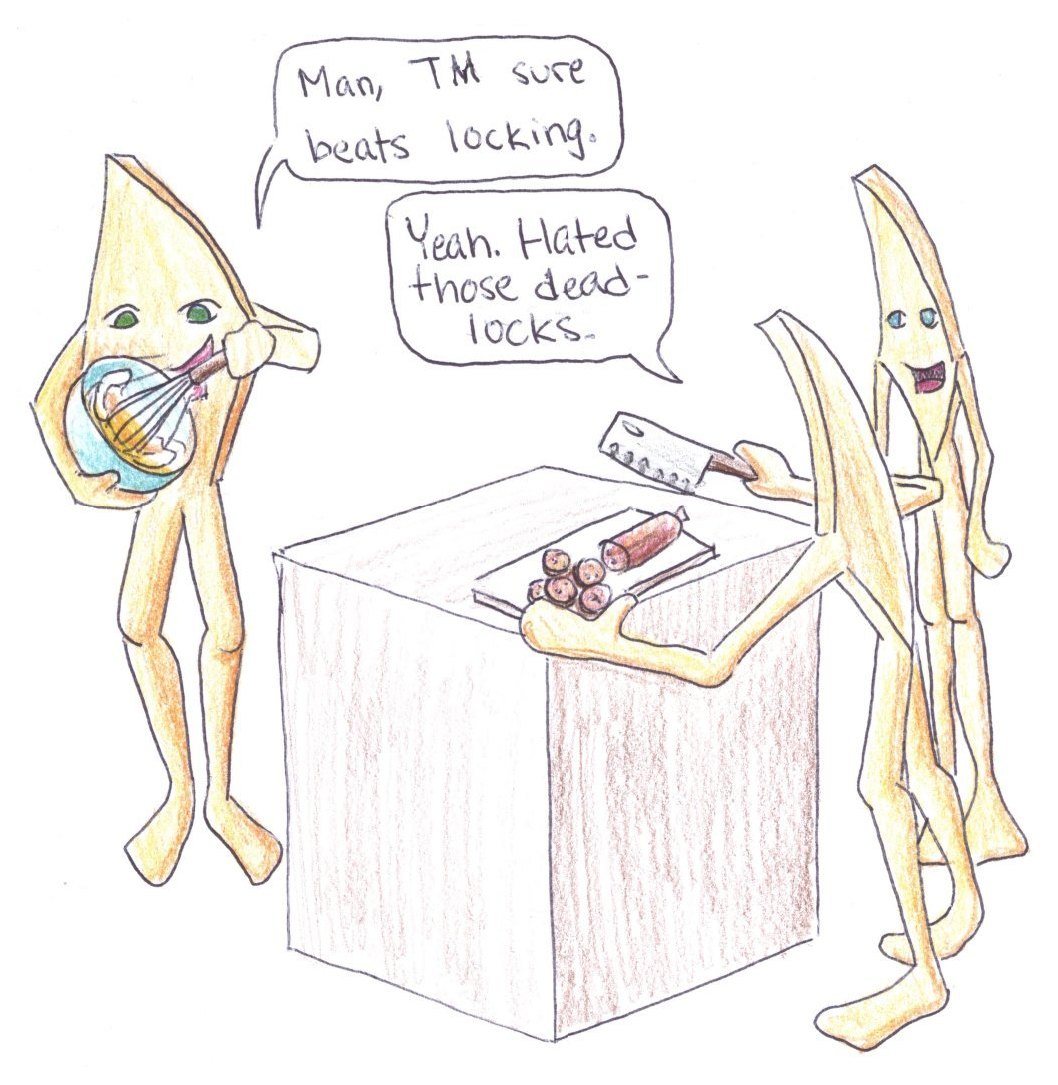
\includegraphics{cartoons/TM-the-vision}}
\end{center}
\caption{The STM Vision}
\ContributedBy{Figure}{fig:future:The STM Vision}{Melissa Broussard}
\end{figure}

\begin{figure}[tb]
\begin{center}
\resizebox{3in}{!}{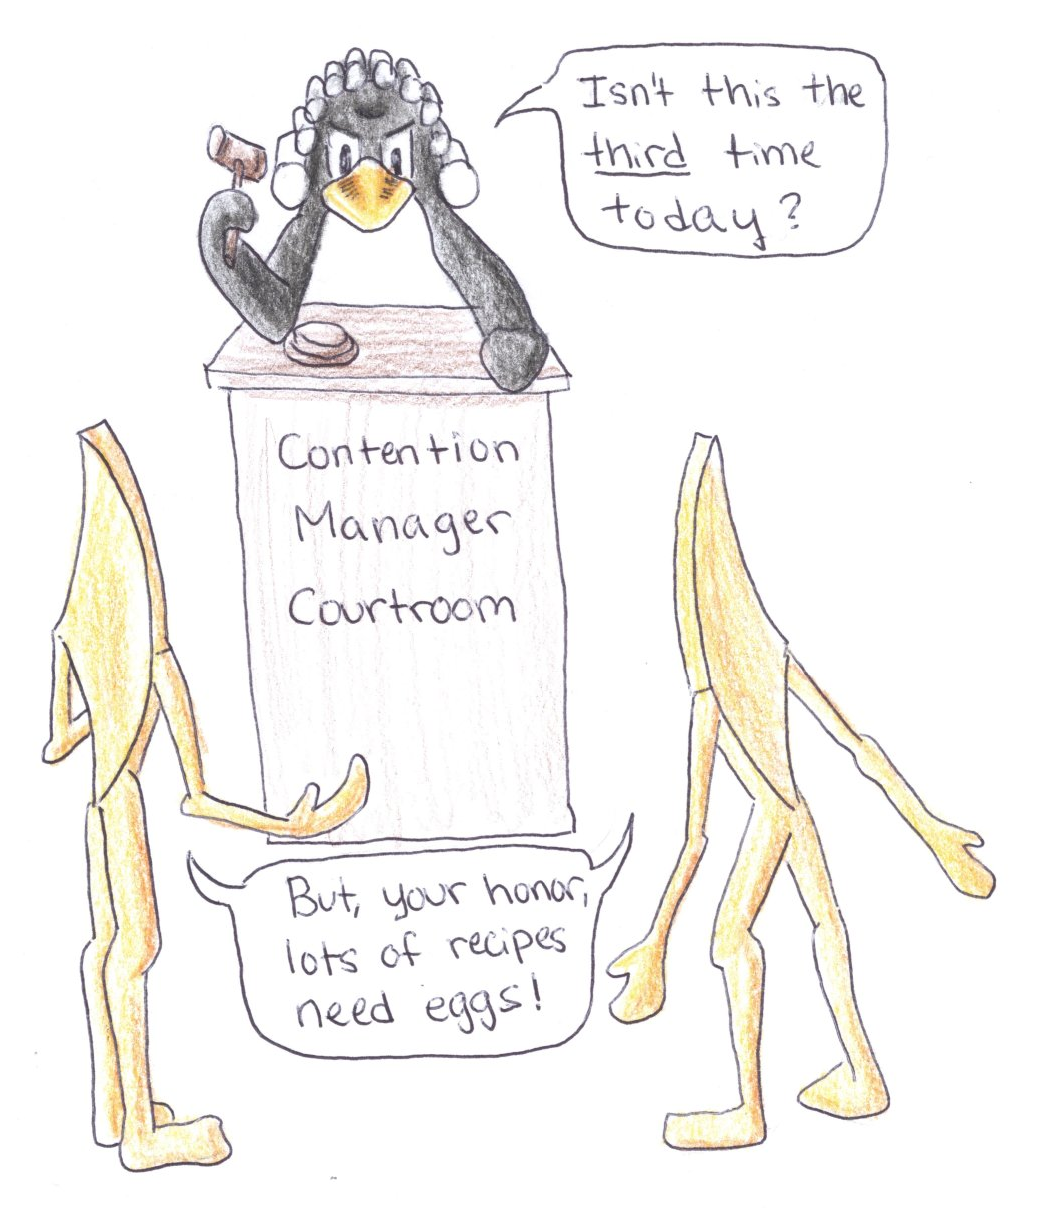
\includegraphics{cartoons/TM-the-reality-conflict}}
\end{center}
\caption{The STM Reality: Conflicts}
\ContributedBy{Figure}{fig:future:The STM Reality: Conflicts}{Melissa Broussard}
\end{figure}

\begin{figure}[tb]
\begin{center}
\resizebox{3in}{!}{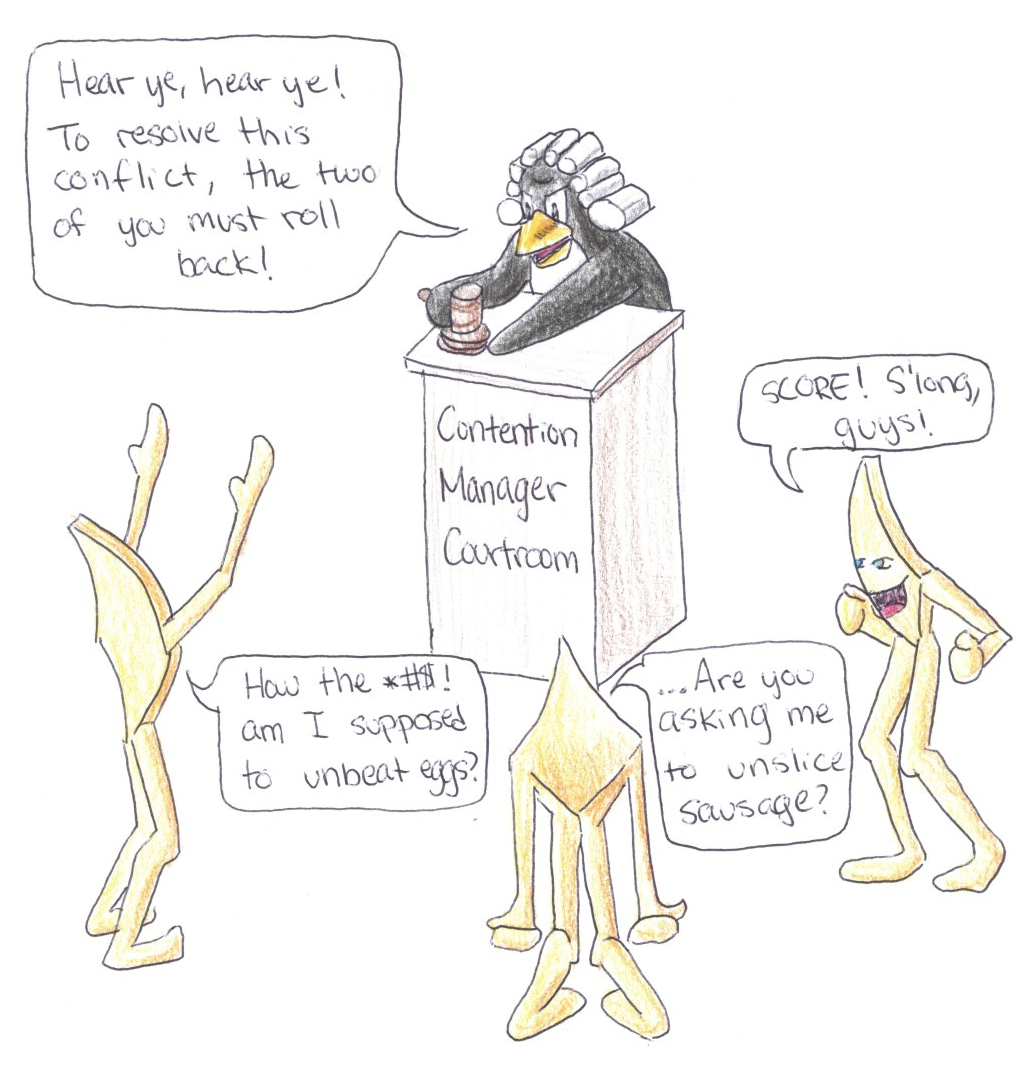
\includegraphics{cartoons/TM-the-reality-nonidempotent}}
\end{center}
\caption{The STM Reality: Irrevocable Operations}
\ContributedBy{Figure}{fig:future:The STM Reality: Irrevocable Operations}{Melissa Broussard}
\end{figure}

\begin{figure}[tb]
\begin{center}
\resizebox{3in}{!}{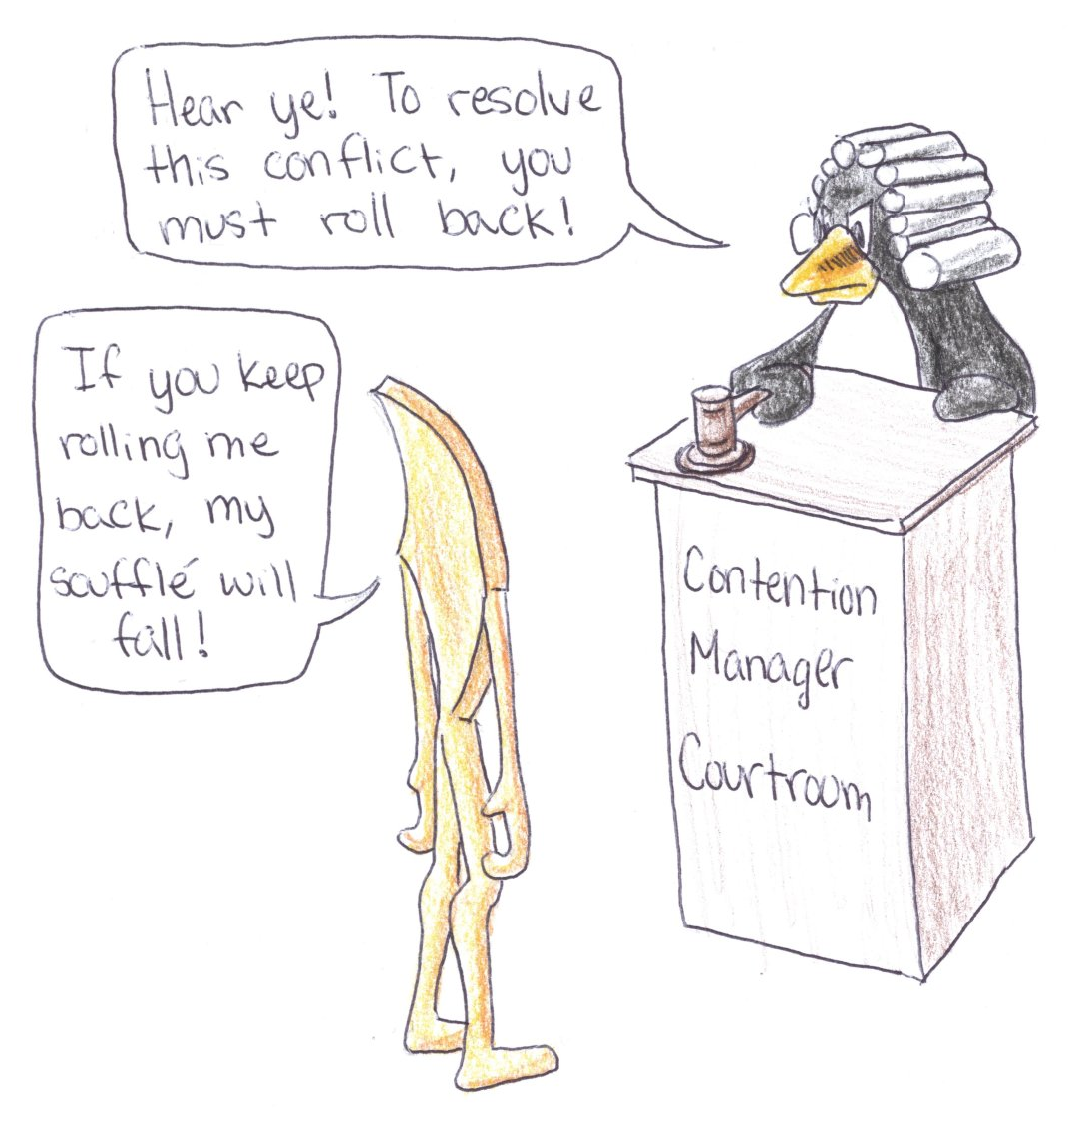
\includegraphics{cartoons/TM-the-reality-realtime}}
\end{center}
\caption{The STM Reality: Realtime Response}
\ContributedBy{Figure}{fig:future:The STM Reality: Realtime Response}{Melissa Broussard}
\end{figure}

But for the moment, the current state of STM
can best be summarized with a series of cartoons.
First,
Figure~\ref{fig:future:The STM Vision}
shows the STM vision.
As always, the reality is a bit more nuanced, as fancifully depicted by
Figures~\ref{fig:future:The STM Reality: Conflicts},
\ref{fig:future:The STM Reality: Irrevocable Operations},
and~\ref{fig:future:The STM Reality: Realtime Response}.

Recent advances in commercially available hardware have opened the door
for variants of HTM, which are addressed in the following section.

% @@@ Don Porter's user-level TM work for Linux.
